\section{Quotienten von Ringen und Moduln}

Seien $M$ und $M'$ zwei $R$-Moduln und $N\subseteq M$ ein Untermodul.

\begin{definition}[Quotientenmodul]
	Für $x\in M$ schreiben wir
	\begin{align}
		x+N:=\{x+y\mid y\in N\}\notag
	\end{align}
	Der \begriff{Quotientenmodul} (oder Faktormodul) von $M$ modulo $N$ ist
	\begin{align}
		\qraum{M}{N}:=\{x+N\mid x\in M\}\notag
	\end{align}
	zusammen mit der Addition
	\begin{align}
		(x+N)+(y+N):=(x+y)+N\quad (x,y\in M)\notag
	\end{align}
	und der Skalarmultiplikation
	\begin{align}
		r\cdot (x+N) := rx+N\quad (x\in M,r\in R)\notag
	\end{align}
	Sei $\pi_N:M\to \qraum{M}{N}$ die Abbildung gegeben durch $x\mapsto x+N$.
\end{definition}

\begin{proposition}[Homomorphiesatz für Moduln]
	\proplbl{8_5_4}
	Sei $f\in\Hom_K(M,M')$ und $N\subseteq M$ ein Untermodul mit $N\subseteq \Ker(f)$. Dann gibt es genau ein $\overline{f}\in\Hom_K(\qraum{M}{N},M')$ mit $f=\overline{f}\circ \pi_N$.
	\begin{center}
		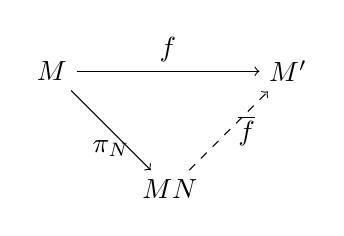
\begin{tikzpicture}
		\node (M) at (0,0) {$M$};
		\node (MS) at (3,0) {$M'$};
		\node (Q) at (1.5,-1.5) {\qraum{$M$}{$N$}};
		\draw[->, above] (M) to node {$f$} (MS);
		\draw[->, below] (M)  to node {$\pi_N$} (Q);
		\draw[->, right, dashed] (Q)  to node {$\overline{f}$} (MS);
		\end{tikzpicture}
	\end{center}
\end{proposition}
\begin{proof}
	Analog zu LAAG 1 III.7.9. Man zeigt, dass jedes $\overline{f}\in\Hom_K(\qraum{M}{N},M')$
	\begin{align}
		\overline{f}(x+N)=f(x)\quad (x\in M)\notag
	\end{align}
	erfüllen muss, und dass dies wiederum eine wohldefinierte Abbildung liefert. %TODO: Verlinkung
\end{proof}

\begin{definition}[Quotientenring]
	Sei $I\unlhd R$ ein Ideal. Für $x\in R$ schreiben wir 
	\begin{align}
		x+I=\{x+a\mid a\in I\}\notag
	\end{align}
	Dann ist
	\begin{align}
		\qraum{R}{I}=\{x+I\mid x\in R\}\notag
	\end{align}
	der \begriff{Quotientenring} von $R$ modulo $I$ mit Addition und Skalarmultiplikation
	\begin{align}
		(x+I)+(x'+I) &= (x+x')+I\quad\forall x,x'\in R \notag \\
		(x+I)\cdot (x'+I) &= (x\cdot x')+I\quad\forall x,x'\in R\notag
	\end{align}
	Und wieder $\pi_I:R\to\qraum{R}{I}$ mit $x\mapsto x+I$.
\end{definition}

\begin{proposition}[Homomorphiesatz für Ringe]
	Sei $\phi:R\to R'$ ein Ringhomomorphismus, $I\unlhd R$ ein Ideal mit $I\subseteq \Ker(\phi)$. Dann gibt es genau einen Ringhomomorphismus mit $\overline{\phi}:\qraum{R}{I}\to R'$, sodass $\overline{\phi}\circ \pi_I=\phi$.
	\begin{center}
		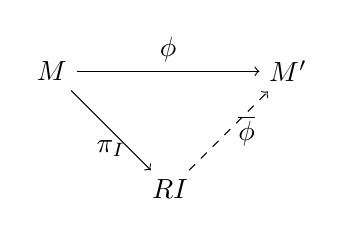
\begin{tikzpicture}
		\node (R) at (0,0) {$M$};
		\node (RS) at (3,0) {$M'$};
		\node (Q) at (1.5,-1.5) {\qraum{$R$}{$I$}};
		\draw[->, above] (R) to node {$\phi$} (RS);
		\draw[->, below] (R)  to node {$\pi_I$} (Q);
		\draw[->, right, dashed] (Q)  to node {$\overline{\phi}$} (RS);
		\end{tikzpicture}
	\end{center}
\end{proposition}
\begin{proof}
	Man sieht, dass 
	\begin{align}
		\overline{\phi}(x+I)=\phi(x)\quad\forall x\in R\notag
	\end{align}
	gelten muss, und das dies auch ein wohldefinierter Ringhomomorphismus ist.
\end{proof}